\documentclass[11pt]{article}
\usepackage[margin=1in]{geometry}
\usepackage{booktabs,graphicx,hyperref,amsmath}
\title{GS-Fuse on Screened C1: Final Report Working Draft}
\author{CMU 11-785 Team 23 \quad (author list to confirm)}
\date{Working draft; not a submission}
\begin{document}
\maketitle
\section{Question and scope}
Does event text improve forecasting when training and test price windows are
separated and suspect article dates are screened? We study the price-task
reference, the return-task redesign, and controlled fusion extensions.
Only the screened price result below is currently collected in this draft.
Historical split results must remain separately identified.
\section{Data and protocol}
The frozen screened C1 protocol retains 6,167 training, 2,302 validation and
2,236 test events after excluding 883 suspect articles. Its emitted input and
target windows were audited for cross-split overlap, and the transferred snapshot
was content verified. Retained article publication times remain unknown; this
screen is not publication-time certification. The input contains 35 OHLC bars
and the target 140 bars. Further dataset detail and citations are pending.
\section{Completed price reference}
The price model uses training-standardized OHLC values, MOMENT-1-large,
Llama-3.2-1B, cross-attention and a softmax gate. Training used seed 0, batch 8,
two epochs in each of three stages, and one H200. All paired controls use the
same checkpoint and 2,236 test events across 845 distinct dates. Shuffled
results average three draws. The two article-free interventions are zero
article tokens through fusion and fusion bypass into the existing decoder;
neither is an independently trained time-series-only model.
\begin{table}[ht]
\centering\small
\begin{tabular}{rrrrr}
\toprule
Horizon & Real & Shuffled & Zero article & Fusion bypass \\
\midrule
35 & 0.00683383 & 0.00683331 & 0.00675873 & 0.00615099 \\
70 & 0.00755942 & 0.00755887 & 0.00749133 & 0.00698376 \\
140 & 0.01137609 & 0.01137603 & 0.01133556 & 0.01115690 \\
\bottomrule
\end{tabular}

\caption{Cumulative-prefix mean squared error in standardized price units,
averaged over OHLC channels and all 2,236 test examples. Lower is better.
The two article-free columns are distinct inference interventions.}
\end{table}
\begin{figure}[ht]
\centering
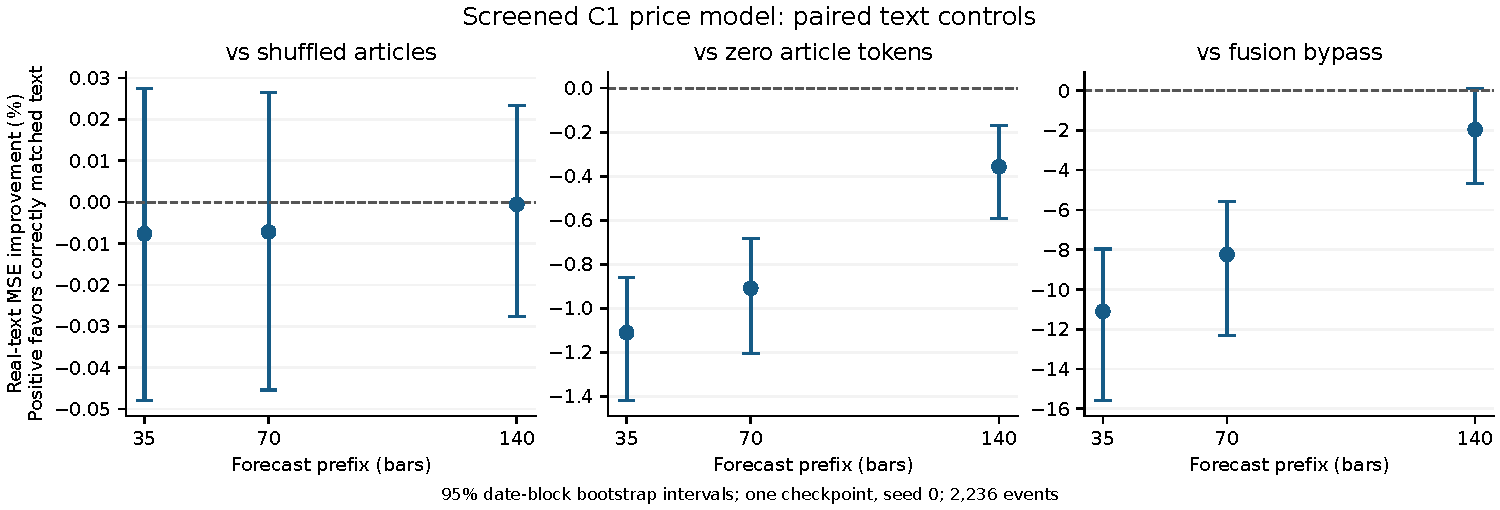
\includegraphics[width=\linewidth]{../../results/screened-price-v1/text-control-gains.pdf}
\caption{Paired real-text MSE improvement relative to each named control.
Positive values favor correctly matched text. Intervals use 1,000 date-block
bootstrap replicates and 20-date blocks, conditional on one checkpoint and
three shuffle draws. Each panel uses its own vertical scale.}
\end{figure}
Correct and shuffled articles have nearly identical MSE at all three horizons;
their improvement intervals include zero. This run therefore provides no
observed matching advantage for this checkpoint. At horizon 140, real-text
MSE is 0.01137609 and shuffled-text MSE is 0.01137603. This does not establish
that financial text is generally useless. Directional accuracy and subgroup
results need their own analysis before they support claims.
\section{Return components and architecture comparisons: pending}
Adaeze owns R0--R3: add forecast direction loss, then full-task gate supervision,
then the learnable last-value shortcut, one change at a time. Jessica owns
Q-Former and Joye owns MoE comparisons. Insert verified result packs here when
available. Architecture variants require a matched R3 reference on the same
data, seed, budget and hardware/environment. The price reference cannot fill
that role. Do not compare standardized-price MSE and basis-point return MSE
directly; use aligned examples and common metric units.
\section{Limitations and remaining work}
Publication times remain unverified. This collected result uses one training
seed; bootstrap block-length sensitivity remains pending. Shuffle donors can
come from later test dates, so shuffling is a diagnostic placebo. Training-seed
replication, persistence comparisons, verified return results, architecture
comparisons, references and full artifact backups remain to be completed or
linked before stronger conclusions and final submission.
\end{document}
